% \documentclass[border=0]{standalone}
\documentclass[a4paper]{article}
\usepackage[left=0mm,top=5mm,right=0mm,bottom=0mm]{geometry}
\usepackage{tikz}
\begin{document}
\thispagestyle{empty}
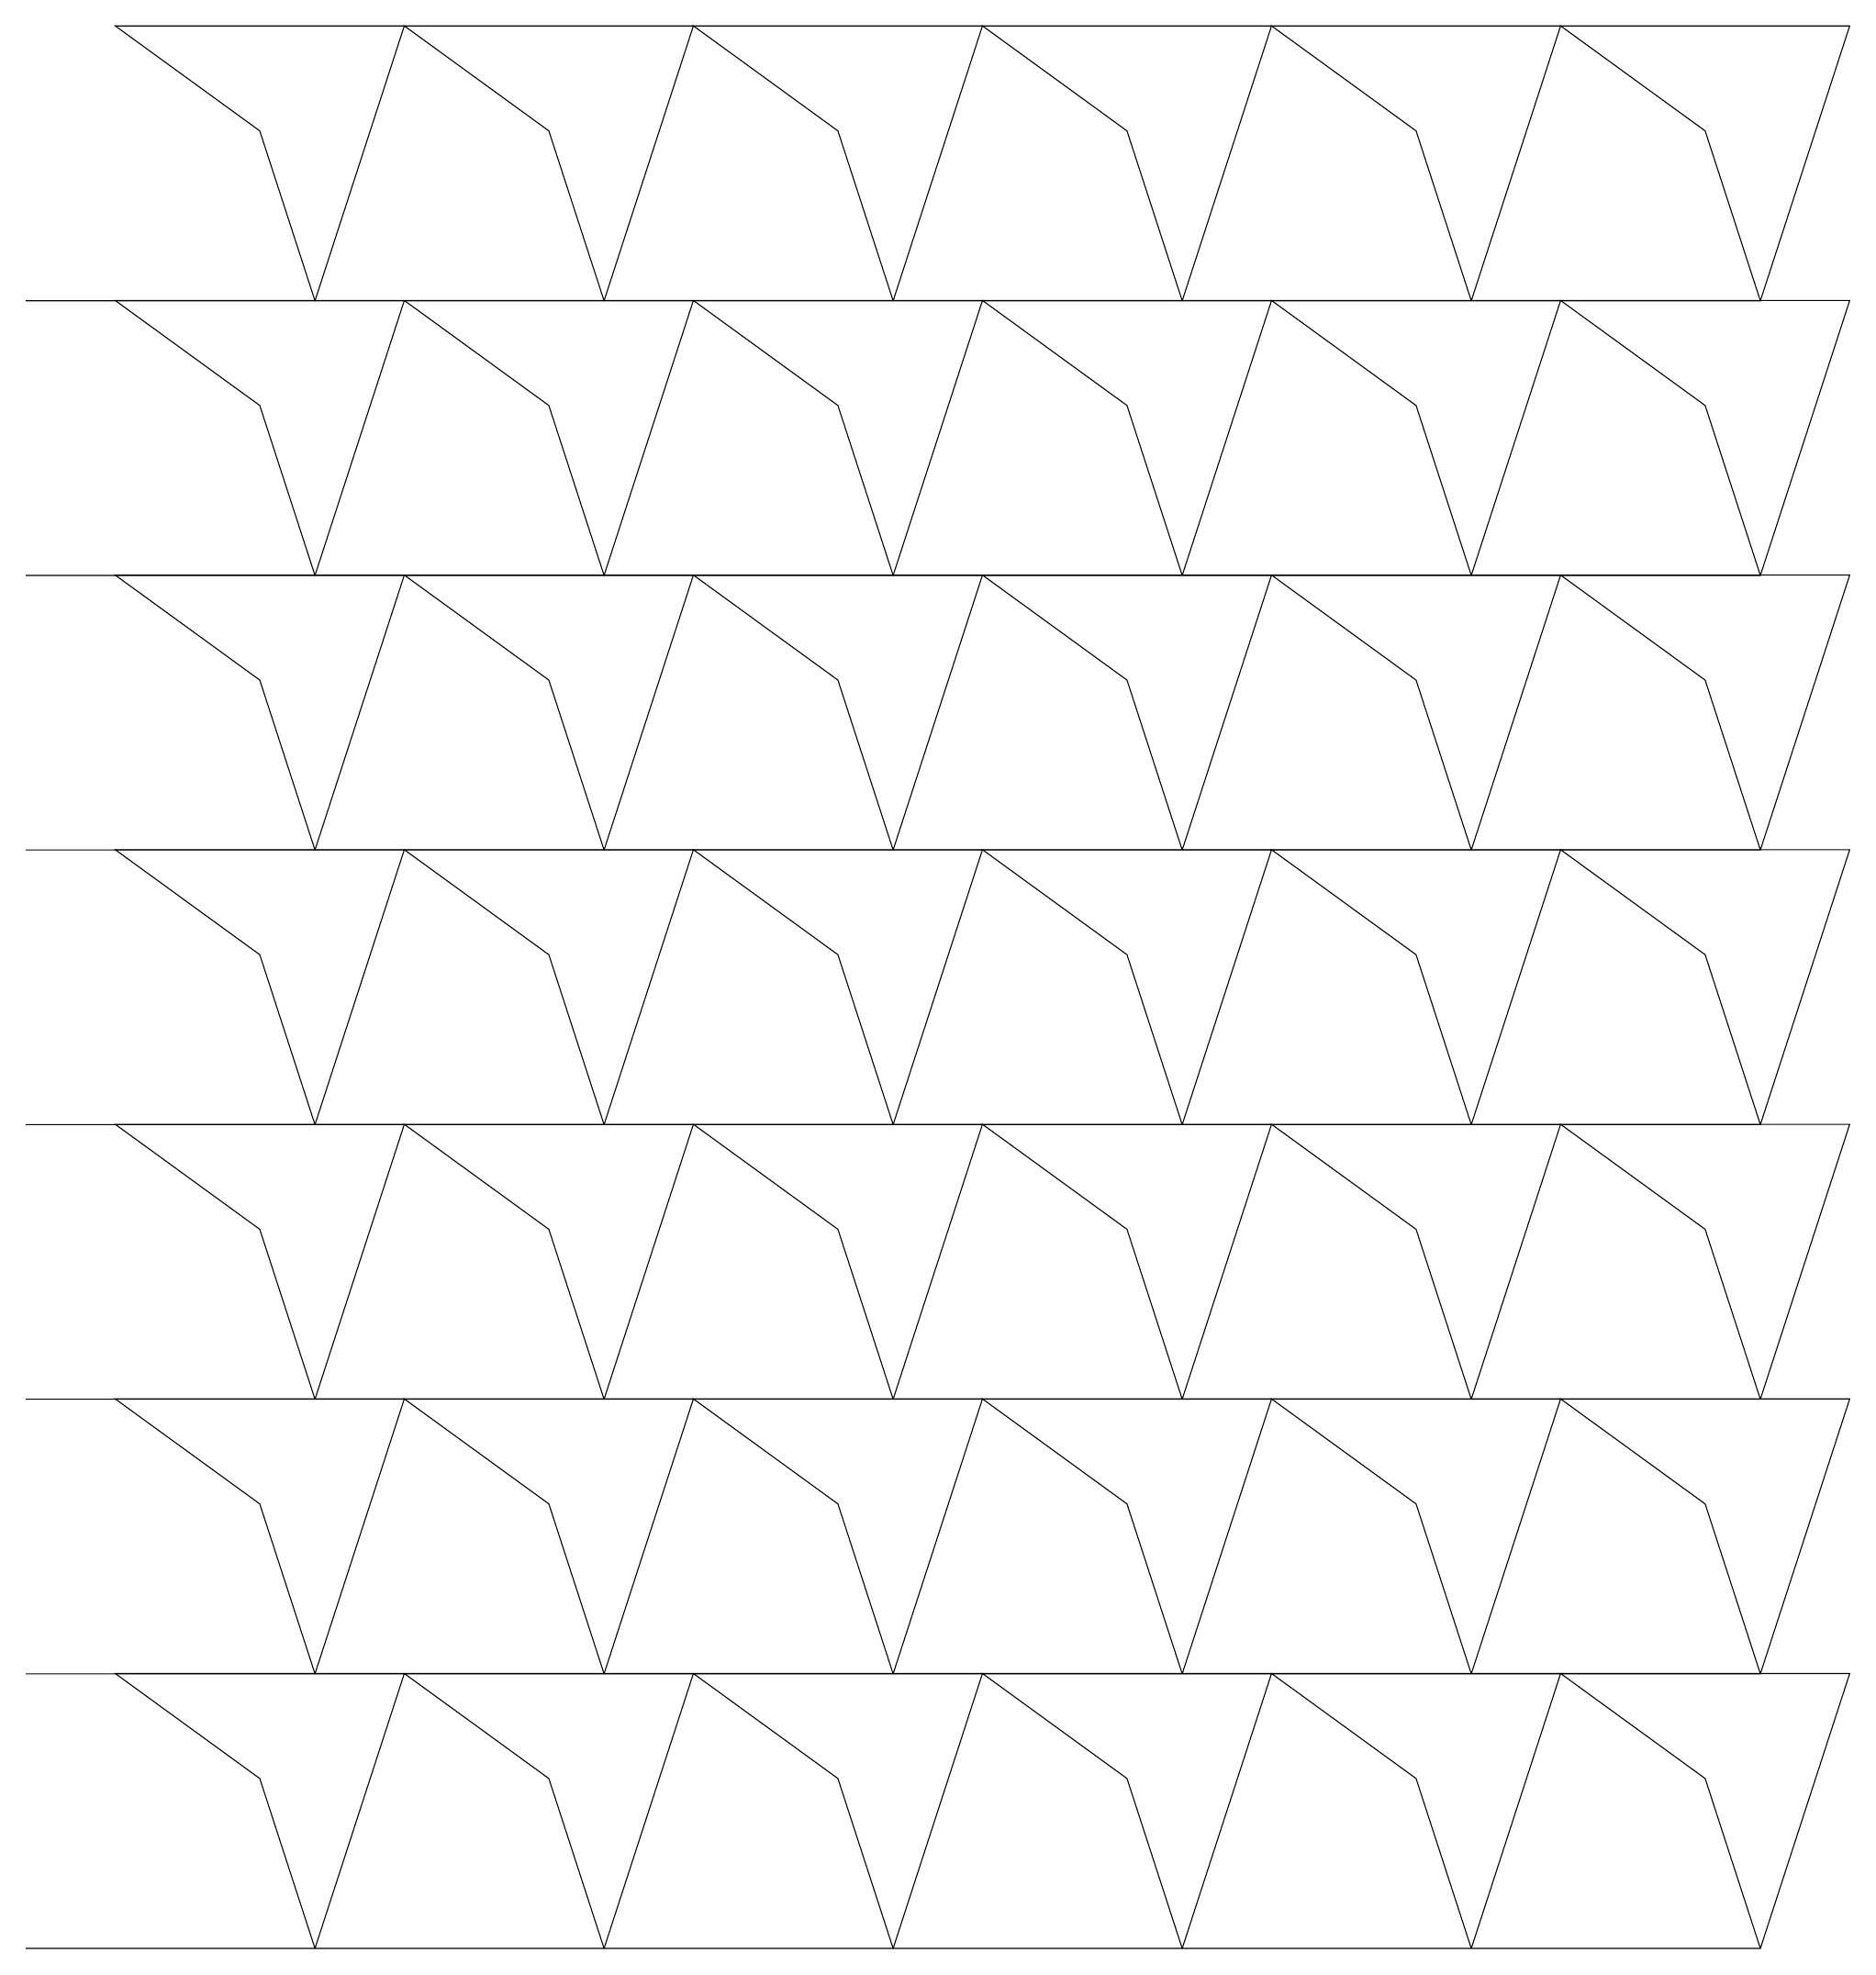
\begin{tikzpicture}
    \pgfmathsetmacro{\p}{(1+sqrt(5))/2}
    \foreach \x in {0,1,2,...,5}{
        \foreach \y in {0,1,...,6}{
            \draw (4*\x,3.8*\y) --++ (0:4)--++(72:4)--++(180:4)--++(-36:4/\p)--++(-72:4/\p);
        }
    }
    % \draw (0,0)--(0:4)--++(72:4)--++(180:4)--(0,0);
    % \draw (72:4) -- (36:4) -- (0:4)--++(72:4);
\end{tikzpicture}
\end{document}